\chapter{Spatial enhancement methods}

\section{Problem statement}

Implement the image enhancement task of Section 3.7 (Fig 3.43) (Section 3.8, Fig 3.46 in our slides).\\
The image to be enhanced is \textit{skeleton\_orig.tif}.\\
You should implement all steps in Figure 3.43. \\
(You cannot directly use functions of Matlab such as
imfilter or fspecial, implement all functions by yourself).

\section{Python implementation}

Usage:~\textbf{python problem2.py [-h] [--laplacian] [--sobel] [-a A] [-g G] [-c C] image\_path}

For example, to run the full image enhancement described in the assignment, using a 3$\times$3 Laplacian filter with A = 1.7,
then a Sobel, a smoothing filter and a Power-Law transformation with c = 1 and gamma = 0.5 type:~\\

\textbf{python problem2.py --laplacian -a 1.7 --sobel -g 0.5 -c 1 skeleton\_orig.tif} \\



\pagebreak
\section{Results}

    \subsection{Original image}

    \begin{figure}[!htb]\centering
        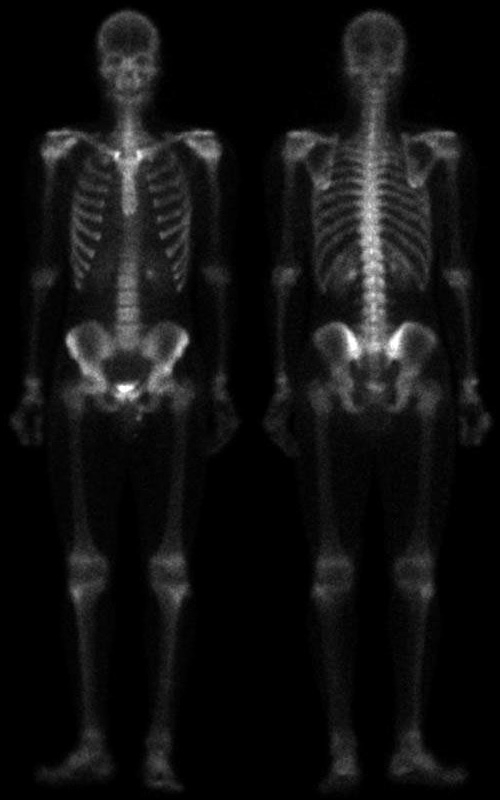
\includegraphics[width=0.7\linewidth]{./images/2/skeleton.jpg}
        \caption{Original \textit{skeleton\_orig.tif}}
        \label{diagram:skeleton}
    \end{figure}


    \pagebreak
    \subsection{3x3 Laplacian (A = 0)}

    \begin{figure}[!htb]\centering
        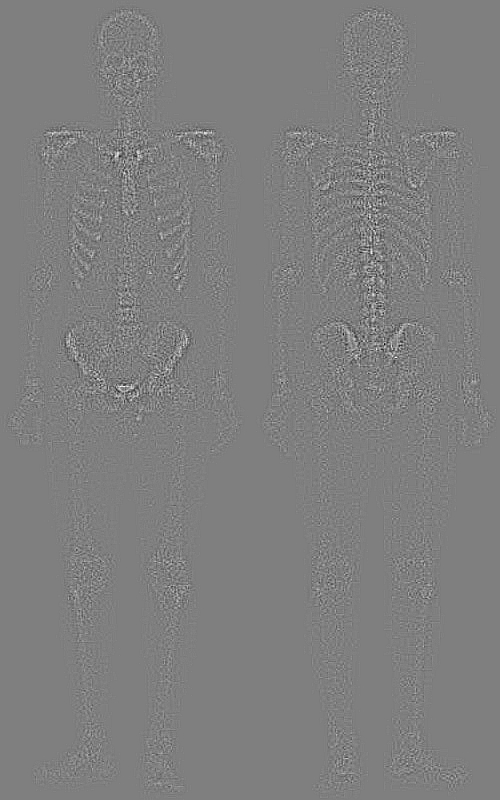
\includegraphics[width=0.4\linewidth]{./images/2/laplacian_A0.jpg}
        \caption{Laplacian (A=0)}\label{diagram:laplacian_0}
    \end{figure}

    \begin{figure}[!htb]\centering
        \begin{minipage}{0.40\textwidth}
            \frame{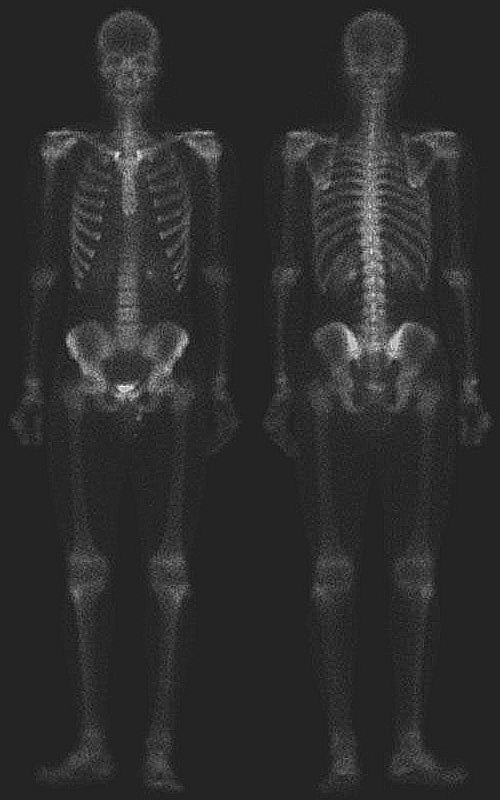
\includegraphics[width=\linewidth]{./images/2/laplacian_A0_sharpened.jpg}}
            \caption{Sharpened image}\label{diagram:laplacian_0_sharpened}
        \end{minipage}
        \begin{minipage}{0.40\textwidth}
        \frame{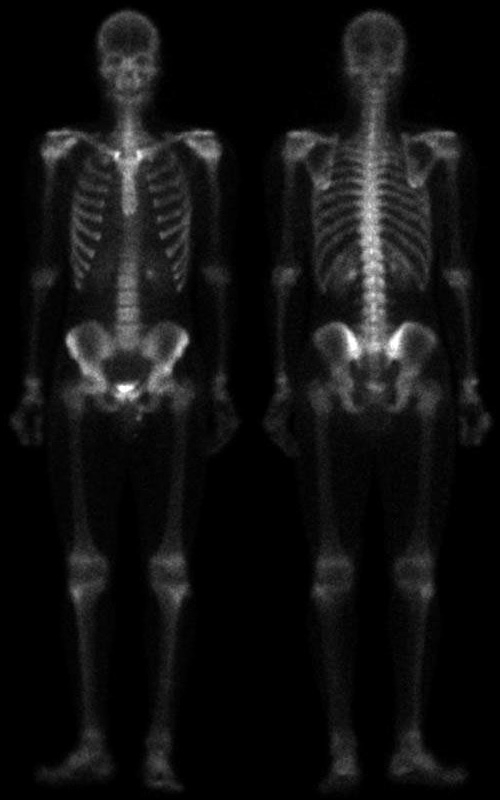
\includegraphics[width=\linewidth]{./images/2/skeleton.jpg}}
        \caption{Original image}
        \end{minipage}
    \end{figure}


    \pagebreak
    \subsection{3x3 Laplacian (A = 1)}

    \begin{figure}[!htb]\centering
        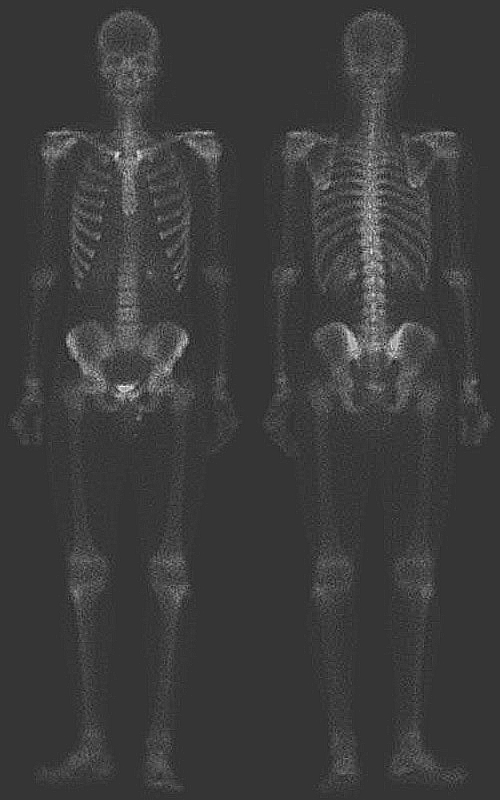
\includegraphics[width=0.4\linewidth]{./images/2/laplacian_A1.jpg}
        \caption{Laplacian (A=1)}\label{diagram:laplacian_1}
    \end{figure}

    \begin{figure}[!htb]\centering
        \begin{minipage}{0.40\textwidth}
            \frame{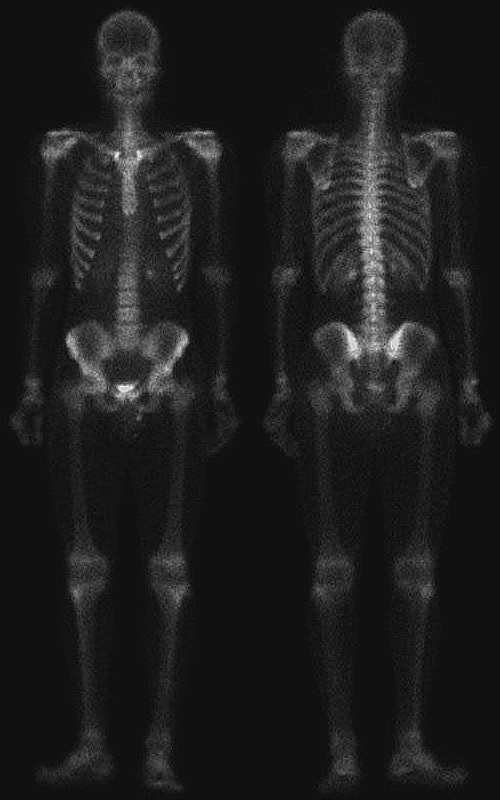
\includegraphics[width=\linewidth]{./images/2/laplacian_A1_sharpened.jpg}}
            \caption{Sharpened image}\label{diagram:laplacian_1_sharpened}
        \end{minipage}
        \begin{minipage}{0.40\textwidth}
        \frame{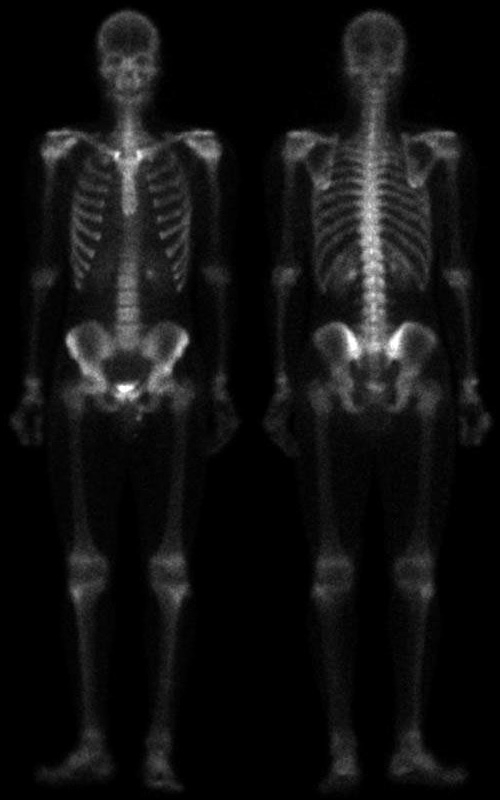
\includegraphics[width=\linewidth]{./images/2/skeleton.jpg}}
        \caption{Original image}
        \end{minipage}
    \end{figure}


    \pagebreak
    \subsection{3x3 Laplacian (A = 1.7)}

    \begin{figure}[!htb]\centering
        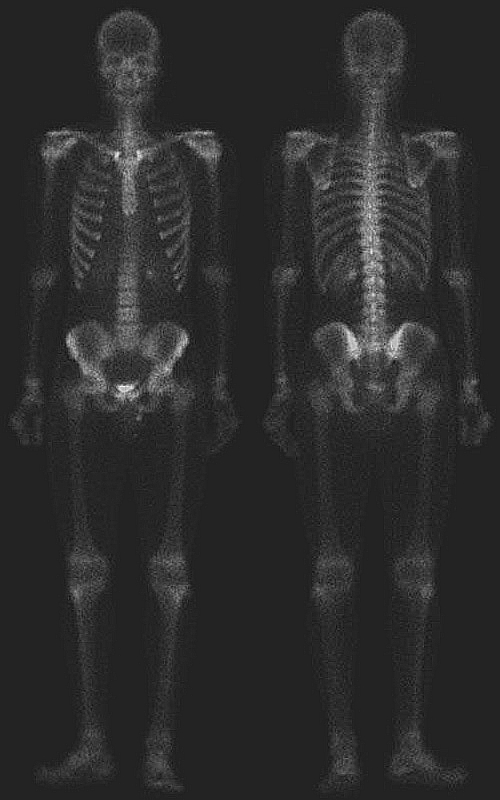
\includegraphics[width=0.4\linewidth]{./images/2/laplacian_A1-7.jpg}
        \caption{Laplacian (A=1.7)}\label{diagram:laplacian_1_7}
    \end{figure}

    \begin{figure}[!htb]\centering
        \begin{minipage}{0.40\textwidth}
            \frame{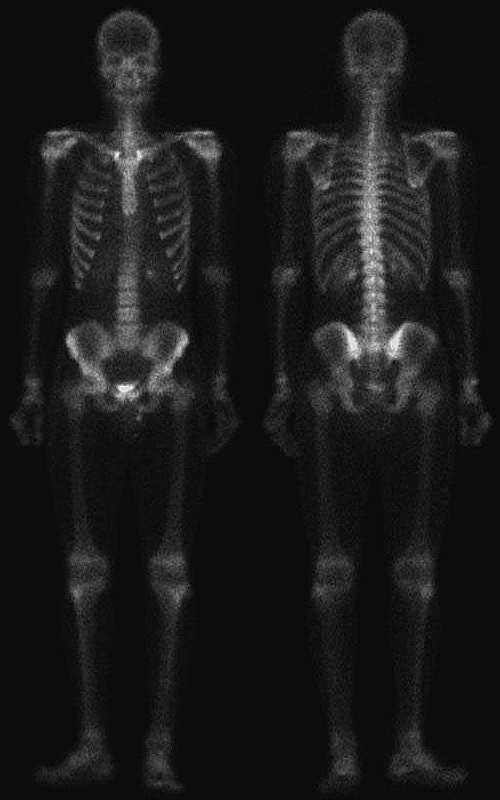
\includegraphics[width=\linewidth]{./images/2/laplacian_A1-7_sharpened.jpg}}
            \caption{Sharpened image}\label{diagram:laplacian_1_7_sharpened}
        \end{minipage}
        \begin{minipage}{0.40\textwidth}
        \frame{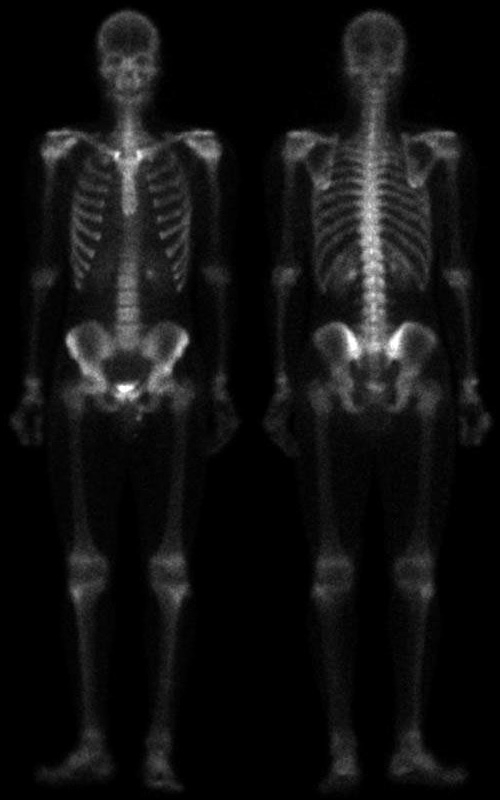
\includegraphics[width=\linewidth]{./images/2/skeleton.jpg}}
        \caption{Original image}
        \end{minipage}
    \end{figure}


    \pagebreak
    \subsection{Sobel}

    \begin{figure}[!htb]\centering
        \begin{minipage}{0.40\textwidth}
            \frame{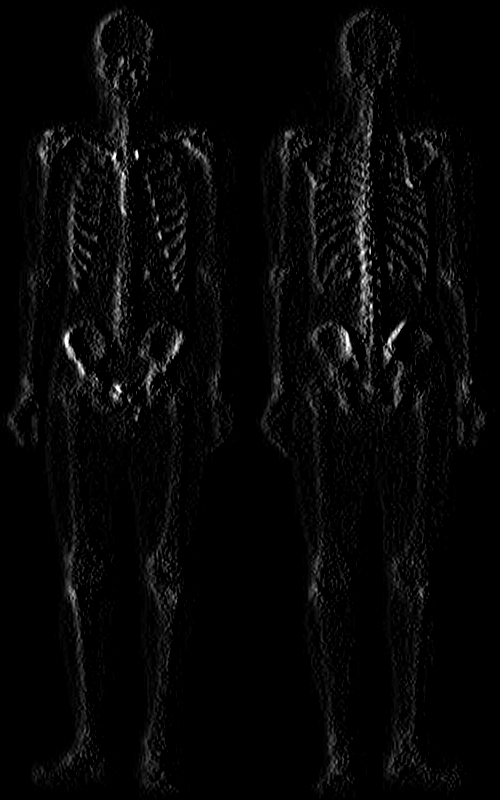
\includegraphics[width=\linewidth]{./images/2/sobel_x_gradient.jpg}}
            \caption{Sobel x-gradient}\label{diagram:sobel_x_gradient}
        \end{minipage}
        \begin{minipage}{0.40\textwidth}
        \frame{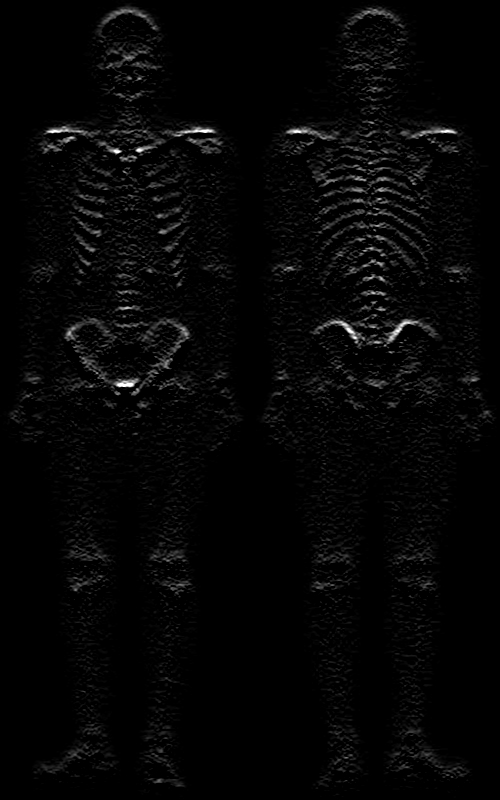
\includegraphics[width=\linewidth]{./images/2/sobel_y_gradient.jpg}}
        \caption{Sobel y-gradient}\label{diagram:sobel_y_gradient}
        \end{minipage}
    \end{figure}

    \begin{figure}[!htb]\centering
        \begin{minipage}{0.40\textwidth}
            \frame{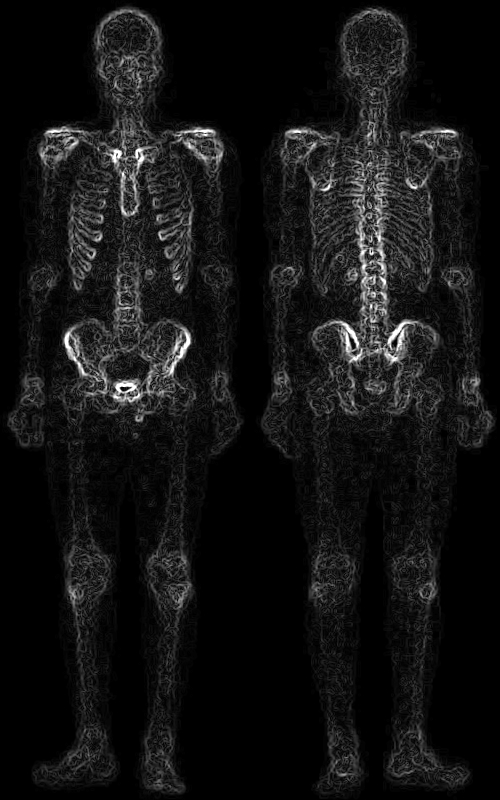
\includegraphics[width=\linewidth]{./images/2/sobel.jpg}}
            \caption{Sobel image}\label{diagram:sobel}
        \end{minipage}
        \begin{minipage}{0.40\textwidth}
        \frame{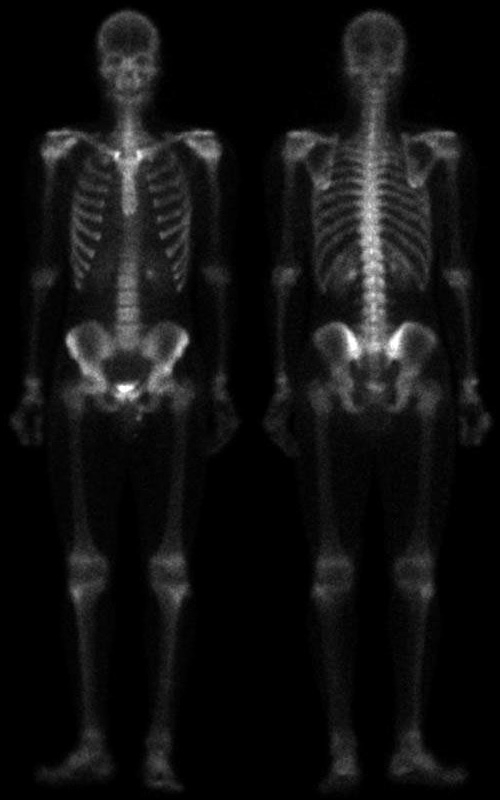
\includegraphics[width=\linewidth]{./images/2/skeleton.jpg}}
        \caption{Original image}
        \end{minipage}
    \end{figure}

    \pagebreak
    \subsection{Smoothing, Sharpening and Power-Law transformation}

    \begin{figure}[!htb]\centering
        \begin{minipage}{0.40\textwidth}
            \frame{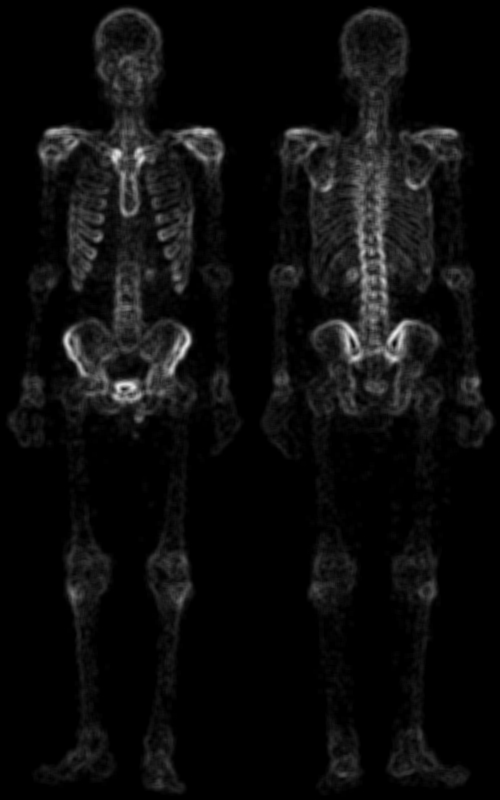
\includegraphics[width=\linewidth]{./images/2/smooth_sobel.jpg}}
            \caption{Smooth Sobel}\label{diagram:smooth_sobel}
        \end{minipage}
        \begin{minipage}{0.40\textwidth}
        \frame{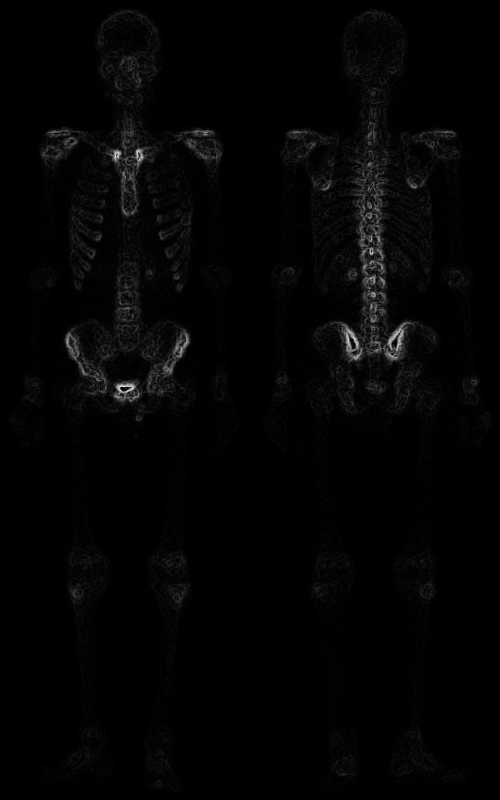
\includegraphics[width=\linewidth]{./images/2/laplacian_x_smooth_sobel.jpg}}
        \caption{Laplacian x Sobel}\label{diagram:laplacian_x_smooth_sobel}
        \end{minipage}
    \end{figure}

    \begin{figure}[!htb]\centering
        \begin{minipage}{0.40\textwidth}
            \frame{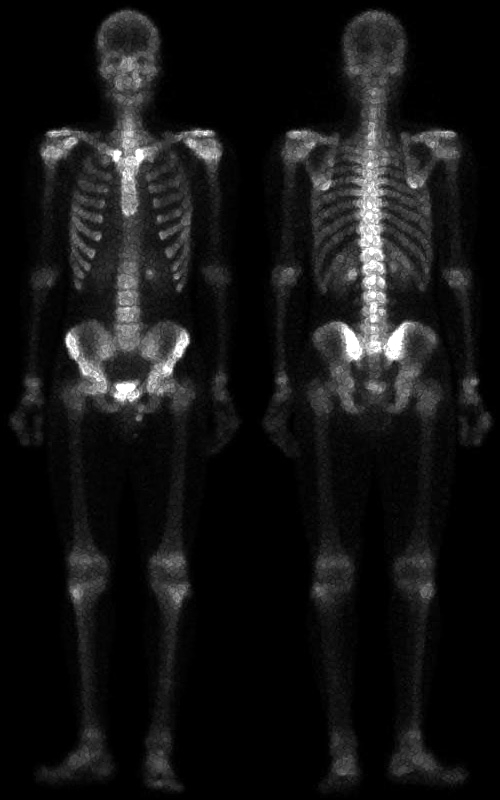
\includegraphics[width=\linewidth]{./images/2/original_+_laplacian_sobel.jpg}}
            \caption{Original + Laplacian x Smooth Sobel}\label{diagram:original_laplacian_sobel}
        \end{minipage}
        \begin{minipage}{0.40\textwidth}
        \frame{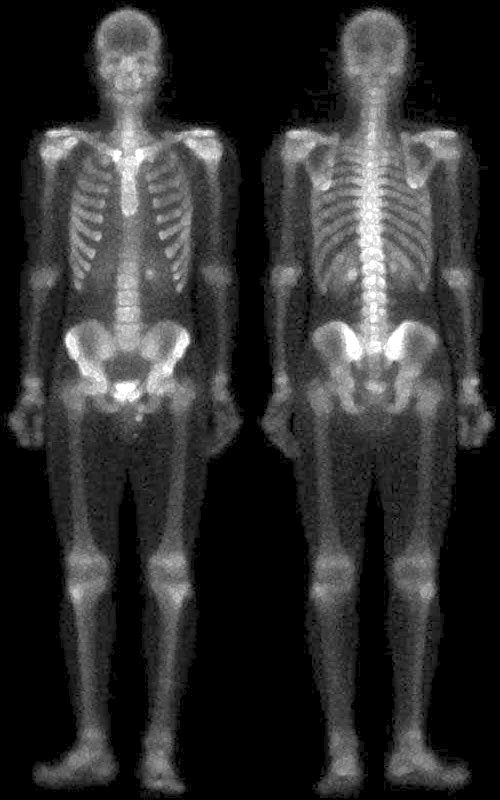
\includegraphics[width=\linewidth]{./images/2/final_image.jpg}}
        \caption{Final image (after Power-Law (c=1, g=0.5))}\label{diagram:final_image}
        \end{minipage}
    \end{figure}


    \pagebreak
    \subsection{Comparison}
    \begin{figure}[!htb]\centering
        \begin{minipage}{0.40\textwidth}
            \frame{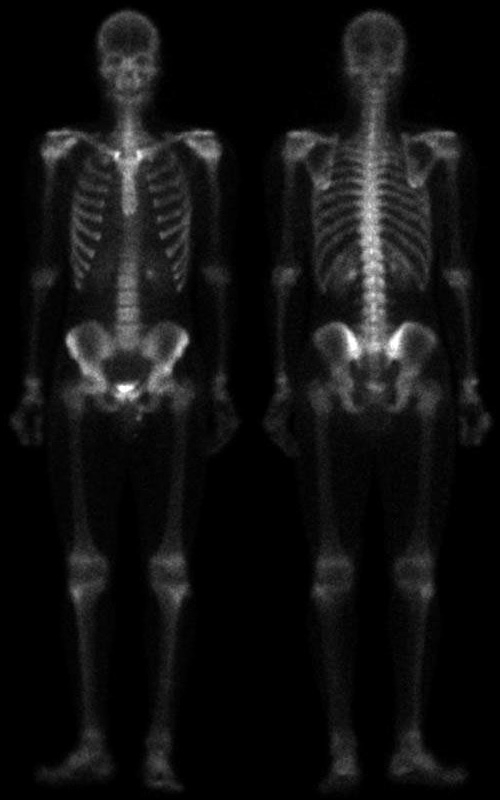
\includegraphics[width=\linewidth]{./images/2/skeleton.jpg}}
            \caption{Original}
        \end{minipage}
        \begin{minipage}{0.40\textwidth}
        \frame{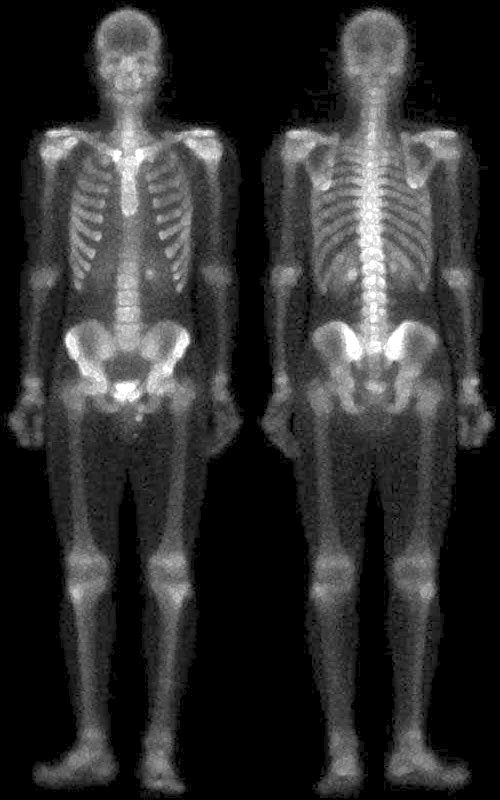
\includegraphics[width=\linewidth]{./images/2/final_image.jpg}}
        \caption{Final image}
        \end{minipage}
    \end{figure}
